\documentclass[12pt]{article}
\title{ECE 141 Homework 4}
\usepackage{subcaption}
\author{Lawrence Liu}
\usepackage{graphicx}
\usepackage{amsmath}
\usepackage{placeins}
\newcommand{\Laplace}{\mathscr{L}}
\setlength{\parskip}{\baselineskip}%
\setlength{\parindent}{0pt}%
\usepackage{xcolor}
\usepackage{listings}
\definecolor{backcolour}{rgb}{0.95,0.95,0.92}
\usepackage{amssymb}
\lstdefinestyle{mystyle}{
    backgroundcolor=\color{backcolour}}
\lstset{style=mystyle}

\begin{document}
\maketitle
\section*{Problem 1}
We have that $$\beta=\arctan(\frac{l_r}{l_r+l_f}\tan(u))$$
therefore
$$\tan(\beta)=\frac{l_r}{l_r+l_f}\tan(u)$$
therefore since the range of $\tan$ is $-\infty$ to $\infty$ for any $\beta$ we can find a $u$ that satisfies the equation.

\section*{Problem 2}
We have that
$$\frac{d}{dt}y=v\sin(\psi+\beta)$$
$$\frac{d}{dt}\psi=\frac{v}{l_R}\sin(\beta)$$
$$\beta=\arctan(\frac{l_r}{l_r+l_f}\tan(u))$$
Linearizing around $\psi=0$ $\beta=0$, we have
$$\frac{d}{dt}y=v(\psi+\beta)$$
$$\frac{d}{dt}\psi=\frac{v}{l_R}\beta$$
therefore taking the laplace transform we have
$$sY=v(\psi+\beta)$$
$$s\psi=\frac{v}{l_r}\beta$$
Therefore we get
$$sY=v(\frac{v}{l_r s}+1)\beta$$
Therefore the transfer function is
$$\frac{Y(s)}{\beta}=\frac{v(v+l_r s)}{l_r s^2}$$
So now with a controller $D_c(s)$ and unity feedback we have that the transfer function is
$$\frac{Y}{R}=\frac{D_c(s)\frac{v(v+l_r s)}{l_r s^2}}{1+D_c(s)\frac{v(v+l_r s)}{l_r s^2}}$$

Letting the controller be a PID controller, we have that the characteristic polynomial is
$$l_r s^3+(k_ps+k_ds^2+k_i)(v^2+l_r v s)=0$$
$$l_r(1+k_d v)s^3+(k_dv^2+l_r v k_p)s^2+(k_pv^2+l_r v k_i)s+v^2k_i=0$$
$$s^3+\frac{(k_dv^2+l_r v k_p)}{l_r(1+k_d v)}s^2+\frac{(k_pv^2+l_r v k_i)}{l_r(1+k_d v)}s+\frac{v^2k_i}{l_r(1+k_d v)}=0$$


Therefore the error is
$$E(s)=R(s)-Y(s)=R(s)-\frac{D_c(s)\frac{v(v+l_r s)}{l_r s^2}}{1+D_c(s)\frac{v(v+l_r s)}{l_r s^2}}R(s)$$
To model a disturbance of length $d$ starting at time $t_1$ and ending at time $t_2$, we let $r(t)=du(t-t_1)-du(t-t_2)$.
and let the controller be a simple $k_p$ controller.

simulating in simulink with $k_p=1$ and $d=1$ and $t_1=4$ and $t_2=6$, we get the following plot for $y(t)$.\\
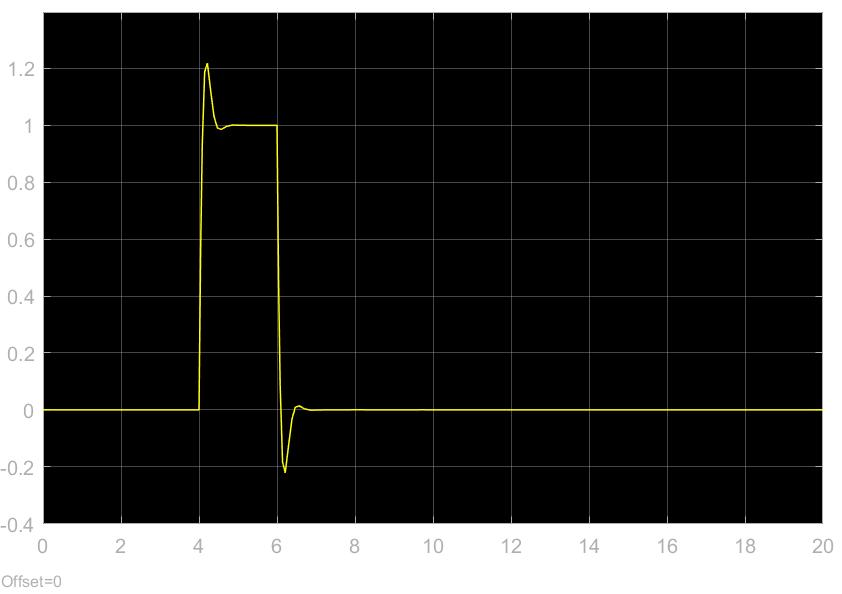
\includegraphics[scale=0.5]{LinearizedProblem1.jpg}
\\As we can see, the controller stabilizes the car at $y=0$.
\end{document}